%!TEX root = ../../Main.tex

\subsection{Задача 2}

Розглянемо також задачу:
%%%
\begin{equation}\label{eq:problem2}
\begin{cases}
	- \Delta u(x_1,x_2) + 10^5 u(x_1, x_2) = f(x_1,x_2), \\
	u|_\Gamma = 0 ,\\
	\Omega = \left[0;1\right] \times \left[0;1\right]
\end{cases}
\end{equation}
%%%

З точним розв'язком
%%
\begin{equation}
	u(x,y) = x_1^{14}x_2(1-x_1)(1-x_2)+x_1 x_2^{14}(1-x_1)(1-x_2),
\end{equation}
%
який зображений на \autoref{plot:problem2_exact}.
%%
\begin{figure}[H]
	\centering
    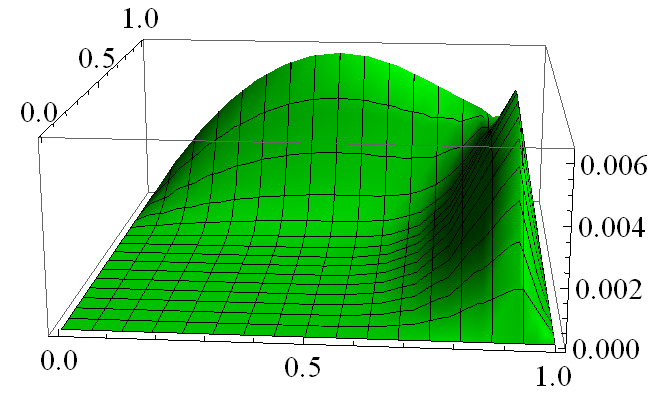
\includegraphics[scale=0.7]{problem2/ExactSolution}
    \captionsetup{format=hang,justification=centering}
    \caption{Точний розв'язок задачі \eqref{eq:problem2}. \newline $u(x_1,x_2) = (1-x_1)(1-x_2)x_1x_2(x_1^{13}+x_2^{13})$ }
    \label{plot:problem2_exact}
\end{figure}

Для адаптивної схеми задамо граничну точність в 7\%, а за початкове розбиття візьмемо рівномірне на сітці 7x7.

Графіки отриманих наближень зображені на \autoref{fig:p2_solution1}-\ref{fig:p2_solution16}:
%
\begin{figure}[H]
	\centering
    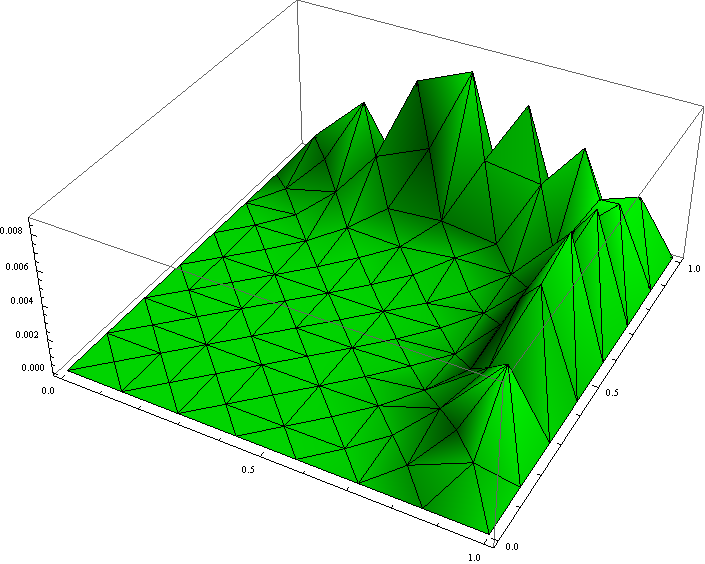
\includegraphics[width=0.8\textwidth]{problem2/my/solutions/solution1}
    \caption{$u_h(x)$ на першому кроці. $N(h) = \nn{196}$.}
    \label{fig:p2_solution1}
\end{figure}
%
\begin{figure}[H]
	\centering
    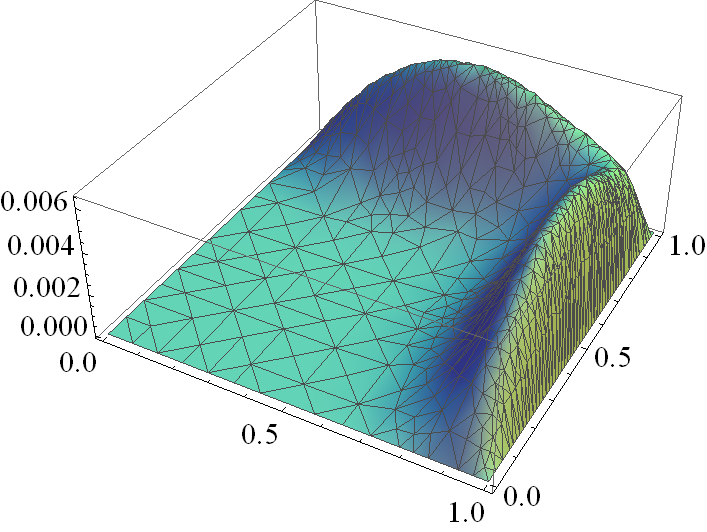
\includegraphics[width=0.8\textwidth]{problem2/my/solutions/solution3}
    \caption{$u_h(x)$ на 3-му кроці. $N(h) = \nn{1293}$.}
    \label{fig:p2_solution3}
\end{figure}
%
\begin{figure}[H]
	\centering
    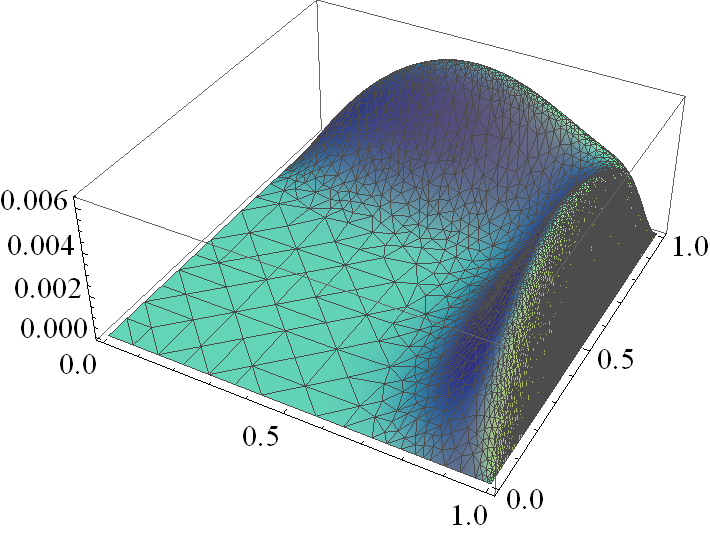
\includegraphics[width=0.8\textwidth]{problem2/my/solutions/solution16}
    \caption{$u_h(x)$ на 16-му кроці. $N(h) = \nn{9519}$.}
    \label{fig:p2_solution16}
\end{figure}

\clearpage
Графіки індикаторів похибок на скінченних елементах зображено на \autoref{fig:p2_aee1}-\ref{fig:p2_aee16}.

\begin{figure}[H]
	\centering
    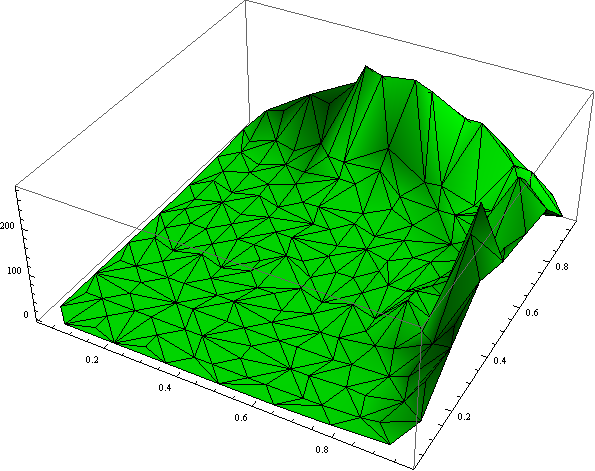
\includegraphics[width=0.7\textwidth]{problem2/my/AEE/aee1}
    \caption{Індикатори похибки на першому кроці. $N(h) = \nn{196}$.}
    \label{fig:p2_aee1}
\end{figure}

\begin{figure}[H]
	\centering
    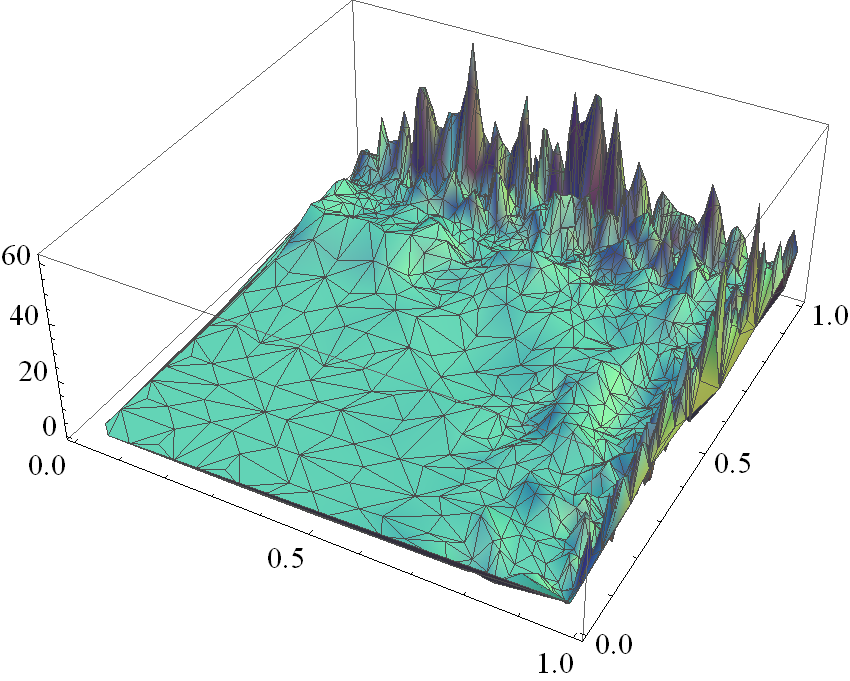
\includegraphics[width=0.7\textwidth]{problem2/my/AEE/aee3}
    \caption{Індикатори похибки на 3-му кроці. $N(h) = \nn{1293}$.}
    \label{fig:p2_aee3}
\end{figure}

\begin{figure}[H]
	\centering
    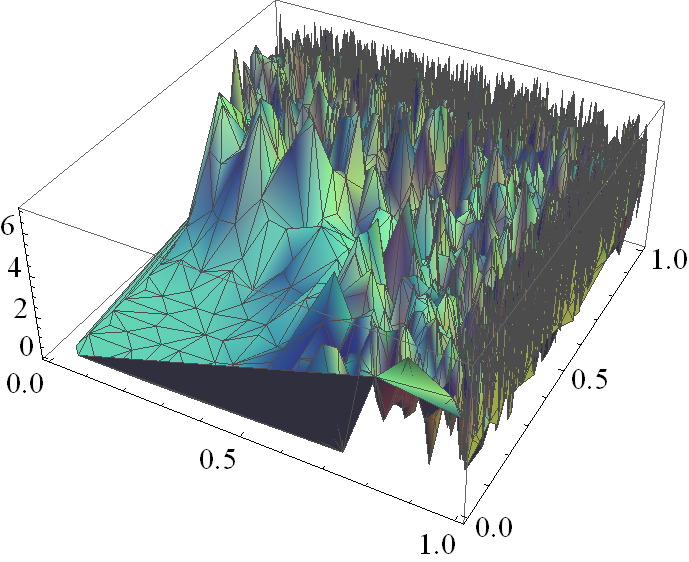
\includegraphics[width=0.7\textwidth]{problem2/my/AEE/aee16}
    \caption{Індикатори похибки на 16-му кроці. $N(h) = \nn{9519}$.}
    \label{fig:p2_aee16}
\end{figure}

Нижче в таблиці наведено деякі показники отриманих розбиття та наближень на кроках адаптивної схеми.
%
\pgfplotstabletypeset[col sep=comma,
	columns={0,1,2,4,5,6,7,3},
	columns/0/.style={
		column name=\textnumero
	},
	columns/1/.style={
		column name=$N(h)$
	},
	columns/2/.style={
		column name=$M(h)$
	},
	columns/3/.style={
		column name=$\norm{e_h^\prime}$
	},
	columns/4/.style={
		column name=$\norm{e_h}$
	},
	columns/5/.style={
		column name=$\norm{e}$
	},
	columns/6/.style={
		column name=${P[u_h]}$,
		fixed,precision=2
	},
	columns/7/.style={
		column name=$\frac{\norm{e_h}}{\norm{e_h+u_h}}\%$,
	},
%%
	begin table=\begin{longtable},
	end table=\end{longtable},
%
	every head row/.style={before row=\caption{Похибки та збіжність схеми.}\\\toprule, after row=\midrule},
	every last row/.style={after row=\bottomrule},
	every nth row={1}{before row=\midrule},
	column type/.add={|}{|}
]{include/8NumResults/problem2/my/errors/table.csv}

Тут:
\begin{equation*}
	\begin{split}
		&\norm{e_h^\prime} \text{ - оцінювач похибки представлений в \cite{OstShynAee11}, } \\
		&\norm{e_h} \text{ - оцінювач похибки представлений в даній роботі,} \\
		&\norm{e} \text{ - реальна похибка,} \\
		&P[u_h]_i = 2\frac{\ln{\norm{e_h^{i-1}}}-\ln{\norm{e_h^i}}}{\ln{N_i}-\ln{N_{i-1}}} \text{ - показник збіжності.} \\
	\end{split}
\end{equation*}
%
Всі норми обраховано в $H_1(\Omega)$. Наведемо також графік збіжності норм похибок.
%
%
\begin{figure}[H]
	\centering
    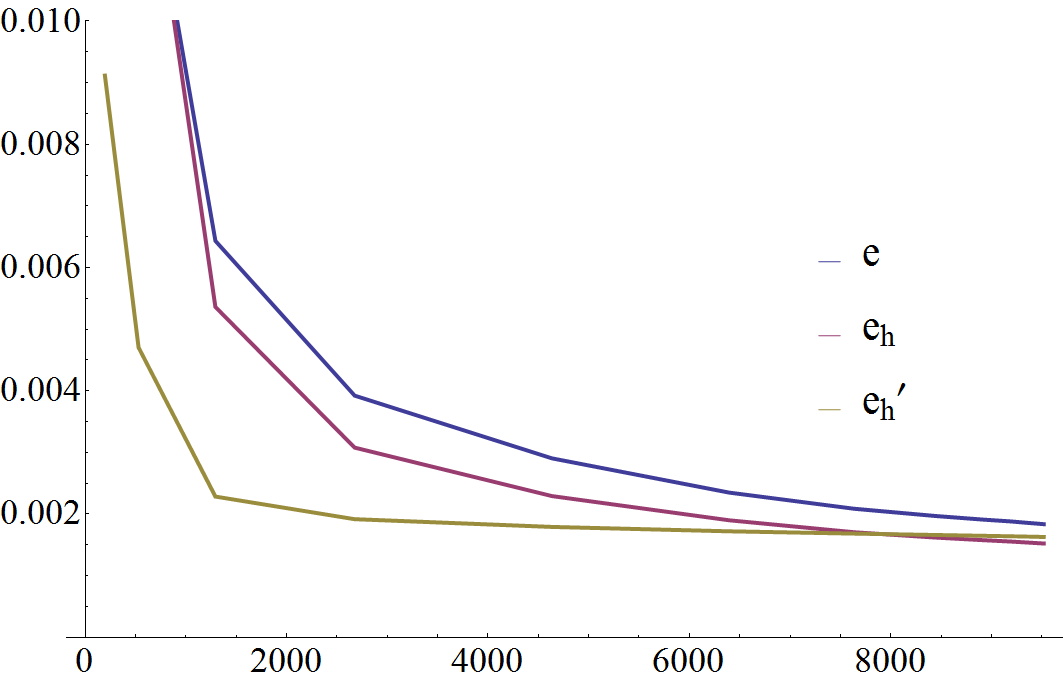
\includegraphics[width=\textwidth]{problem2/my/Plotnb}
    \caption{Збіжність норм похибок МСЕ із збільшенням кількості елементів.}
    \label{fig:p2_my_errors}
\end{figure}

Якщо ж за основу для адаптивної стратегії взяти оцінювач з \cite{OstShynAee11}, то таблиця обчислених результатів матиме вигляд:

\pgfplotstabletypeset[col sep=comma,
	columns={0,1,2,3,5,6,7,4},
	columns/0/.style={
		column name=\textnumero
	},
	columns/1/.style={
		column name=$N(h)$
	},
	columns/2/.style={
		column name=$M(h)$
	},
	columns/3/.style={
		column name=$\norm{e_h^\prime}$
	},
	columns/4/.style={
		column name=$\norm{e_h}$
	},
	columns/5/.style={
		column name=$\norm{e}$
	},
	columns/6/.style={
		column name=${P[u_h]}$,
		fixed,precision=2
	},
	columns/7/.style={
		column name=$\frac{\norm{e_h}}{\norm{e_h+u_h}}\%$
	},
%%
	begin table=\begin{longtable},
	end table=\end{longtable},
%
	every head row/.style={before row=\caption{Похибки та збіжність схеми.}\\\toprule, after row=\midrule},
	every last row/.style={after row=\bottomrule},
	every nth row={1}{before row=\midrule},
	column type/.add={|}{|}
]{include/8NumResults/problem2/ost/errors/table.csv}

\clearpage
Графік залежності похибки від кількості елементів має вигляд:

\begin{figure}[H]
	\centering
    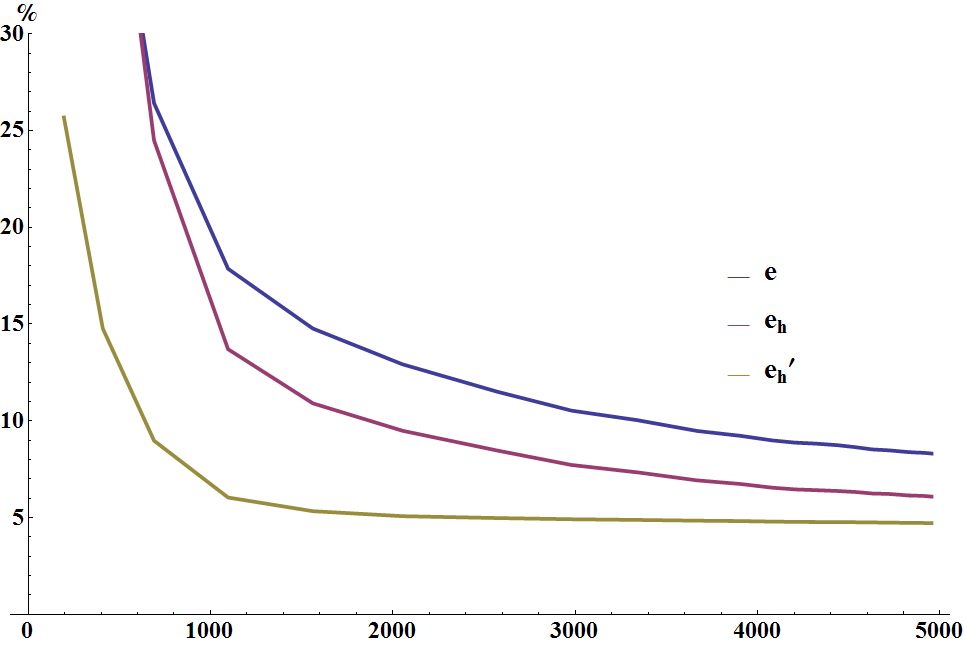
\includegraphics[width=\textwidth]{problem2/ost/Plotnb}
    \caption{Збіжність норм похибок із збільшенням кількості елементів.}
    \label{fig:p2_ost_errors}
\end{figure}
Оцінювач з \cite{OstShynAee11} використав меншу кількість елементів, ніж оцінювач \eqref{eq:AEE_final} (\nn{4953} проти \nn{9519}). Проте для цього йому знадобилося більше кроків (26 і 16 відповідно). Похибка при цьому оцінена майже вдвічі менше від реальної.

